\chapter{The ATLAS Detector}
\label{chap:atlas}
\section{Overview}
The A Toroidal LHC ApparatuS (ATLAS) is the largest general purpose detector at the LHC.  It is designed to record and reconstruct the products of proton proton collisions over a broad range of energies and final state topologies. The detector combines tracking, calorimetry, and muon detection systems in order to provide precise measurements of charged particle trajectories, particle energies, and event level observables. 

ATLAS is built in a cylindrical geometry around the beam axis, with subdetectors arranged in concentric layers, schematically shown in figure~\ref{fig:atlas_detector}. The coordinate system is defined with its origin at the nominal interaction point. The $z$ axis is aligned with the beam direction, the $x$ axis points from the interaction point toward the centre of the LHC ring, and the $y$ axis points upward. In the plane transverse to the beam, particle directions are described by the azimuthal angle $\phi$. The polar angle $\theta$ with respect to the beam axis is commonly expressed in terms of pseudorapidity $\eta = -\ln\tan(\theta/2)$.

Angular separations in the detector are quantified using the distance measurement $\Delta R = \sqrt{(\Delta\eta)^2 + (\Delta\phi)^2}$. This quantity is important to jet reconstruction, where it defines the angular radius of clustering algorithms.

\begin{figure}[H]
    \centering
    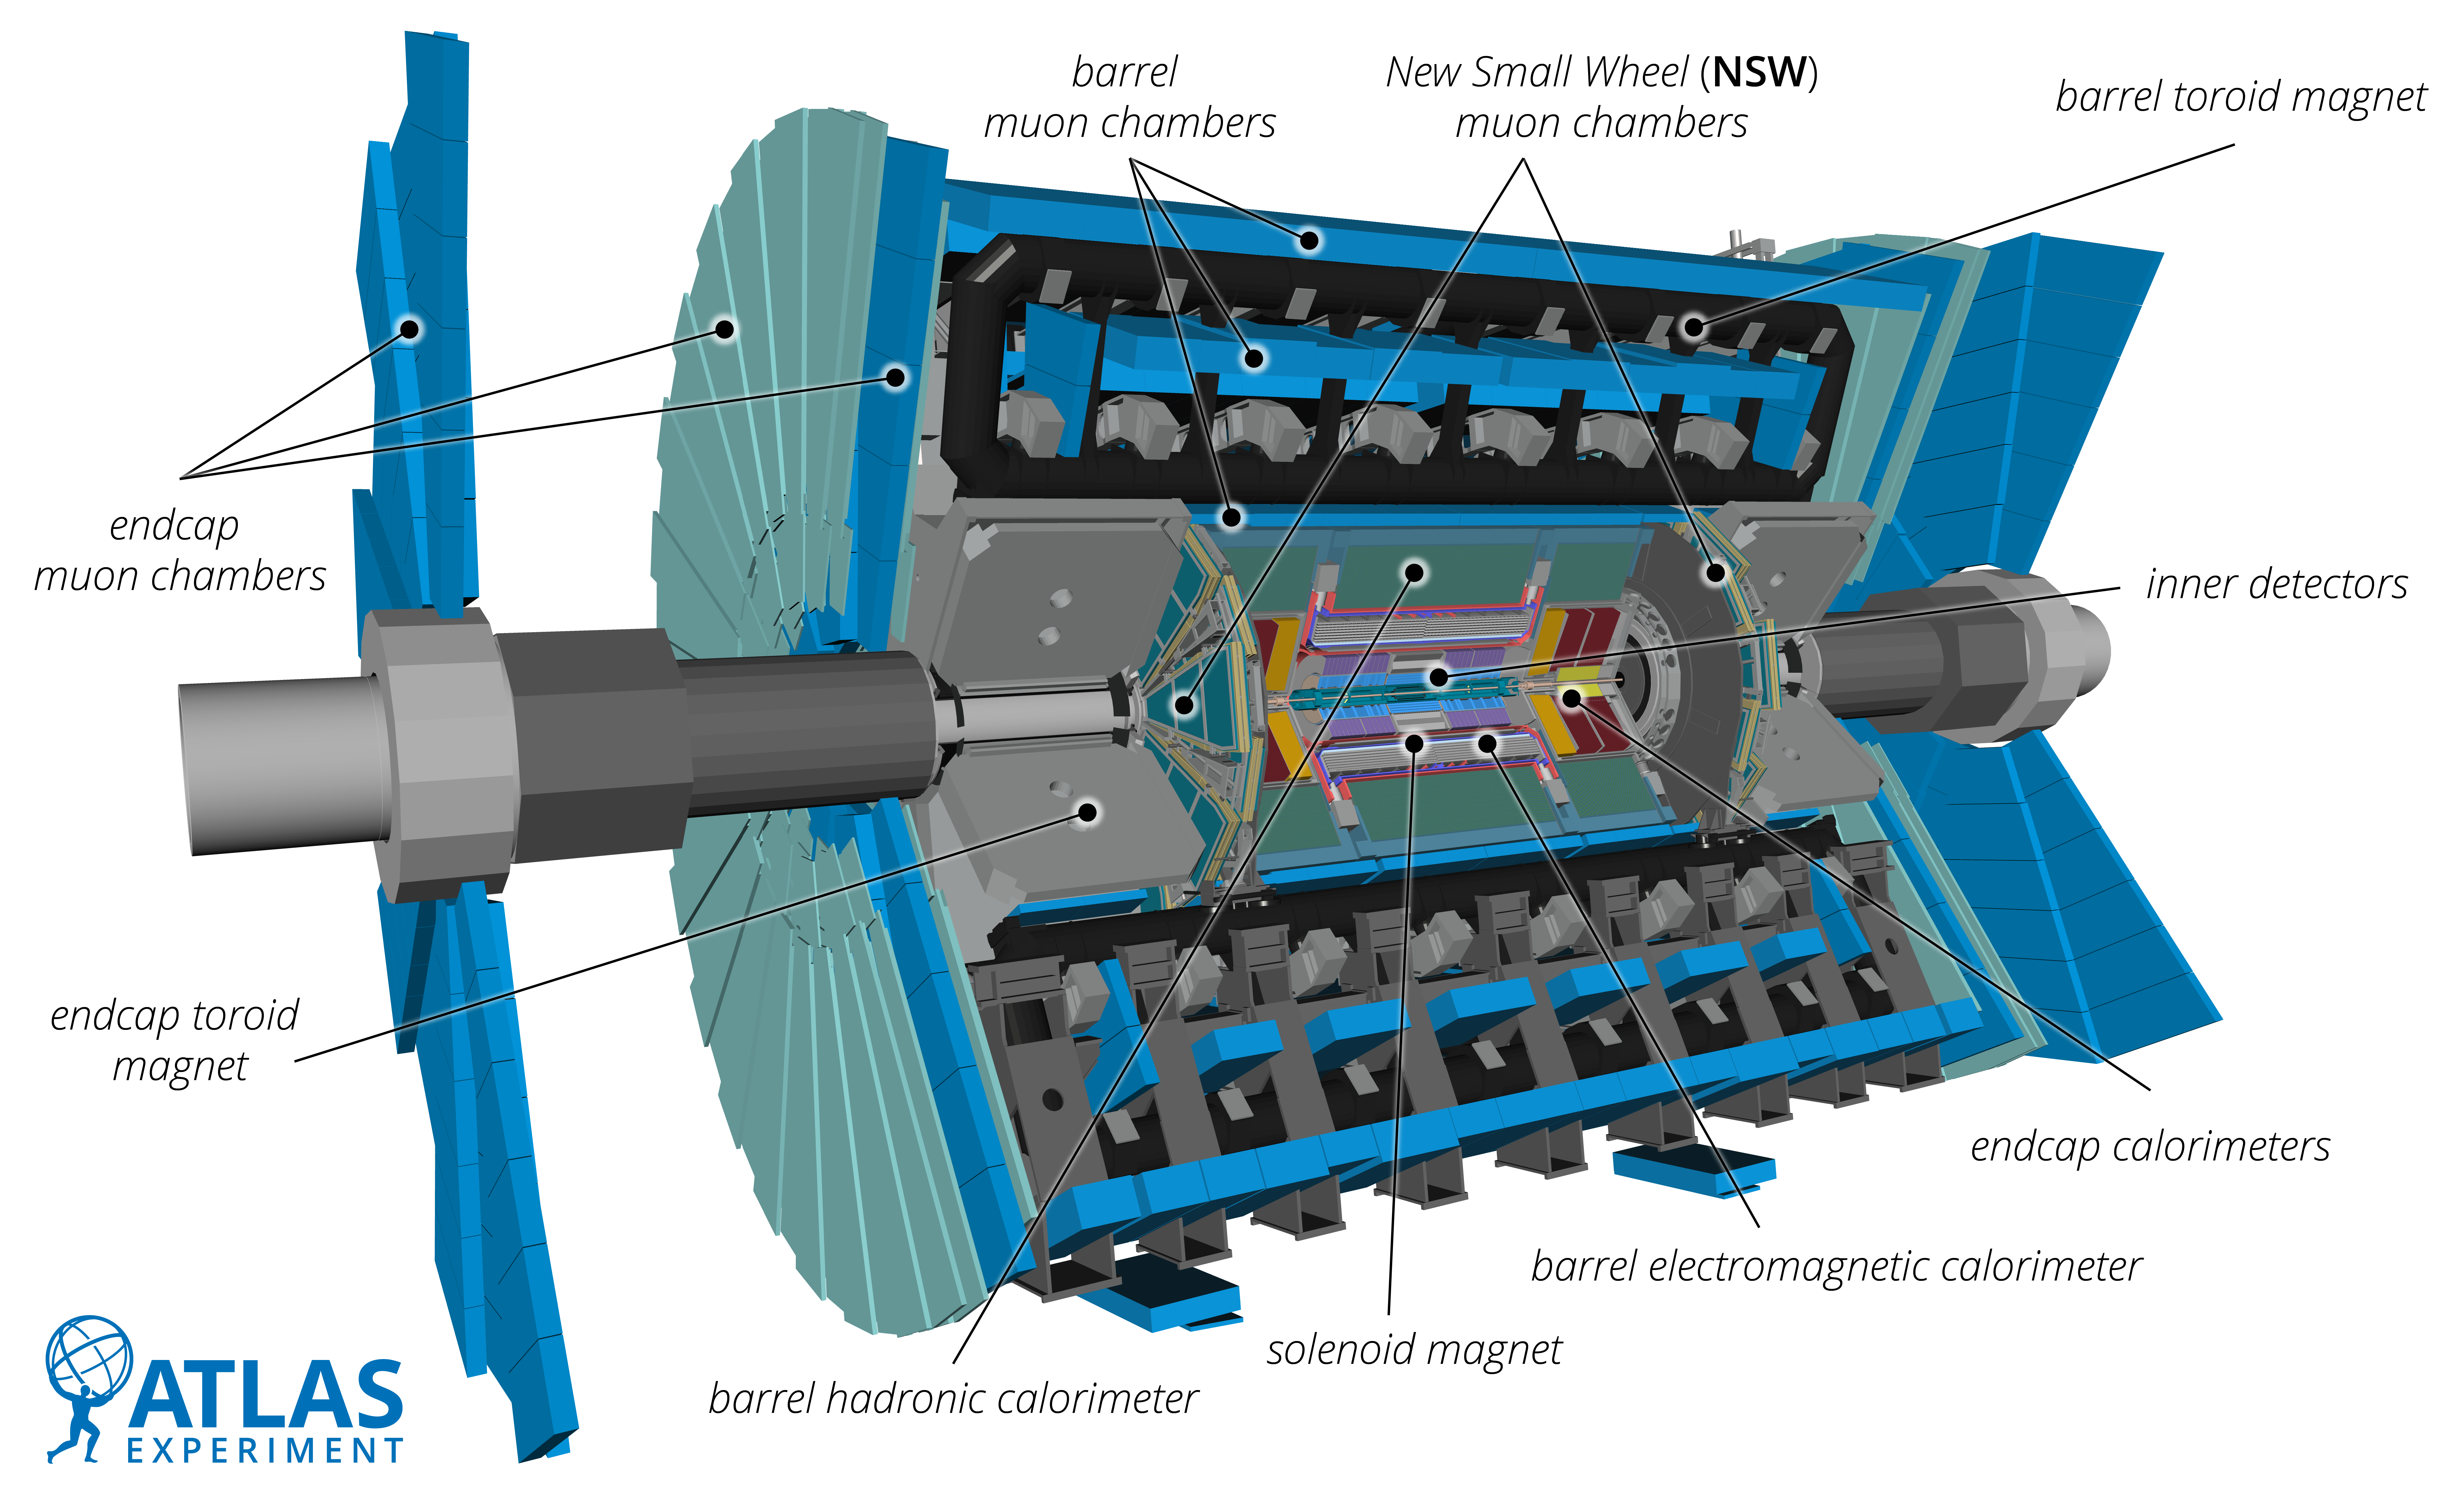
\includegraphics[width=0.86\textwidth]{figures/Detector.png}
    \caption{Schematic overview of the ATLAS detector, showing the inner detector, calorimeter systems, and muon spectrometer arranged concentrically around the interaction point.}
    \label{fig:atlas_detector}
\end{figure}

\section{Large Hadron Collider}
The Large Hadron Collider is a circular proton proton accelerator with a circumference of approximately 27 km, located in an underground tunnel near Geneva. Protons are accelerated through a chain of pre accelerators before being injected into the LHC, where they are guided by superconducting dipole magnets producing magnetic fields of 8.3 T.

During physics operation, the LHC collides two counter rotating proton beams at several interaction points, including the location of the ATLAS detector. Each beam consists of up to several thousand proton bunches, with individual bunches containing of order $10^{11}$ protons and separated by 25 ns.

The data taking history of the LHC is divided into distinct running periods. Run 1, conducted between 2010 and 2012 at centre of mass energies of 7 and 8 TeV, delivered an integrated luminosity of approximately 25 fb$^{-1}$ to ATLAS. Run 2 took place between 2015 and 2018 at a centre of mass energy of 13 TeV and provided a significantly larger dataset corresponding to about 140 fb$^{-1}$. In this analysis, data and simulated events based on run 2 are used.

\section{Inner detector}
The inner detector is responsible for reconstructing the trajectories of charged particles produced in a collision. The system is composed of multiple concentric tracking subsystems arranged around the beam axis to provide high precision spatial measurements over a broad pseudorapidity range, extending to approximately $|\eta| <  2.5$. 

It operates within a solenoidal magnetic field, which causes charged particles to follow curved paths. The magnetic field, with a strength of approximately 2~T, is oriented parallel to the beam axis and is generated by a superconducting solenoid surrounding the tracking volume, ensuring uniform bending of charged particle trajectories in the transverse plane. 

The transverse momentum of the particle can be inferred from this produced curvature. This relationship follows directly from the Lorentz force, where the radius of curvature is proportional to the particle momentum and inversely proportional to the magnetic field strength. 

The inner detector provides measurements close to the interaction point, enabling vertex reconstruction and discrimination between tracks originating from the primary hard scatter and those from additional proton proton interactions in the same bunch crossing, known as as pile up.
\section{Calorimeter system}
Surrounding the inner detector is the calorimeter system, which measures the energy of particles by absorbing them and recording the resulting electromagnetic and hadronic showers. As particles traverse dense absorber material, they initiate cascades of secondary particles, and the total deposited energy is sampled by active detector elements. The calorimeter coverage extends over a wide pseudorapidity range, around $|\eta| < 4.9$

The electromagnetic calorimeter is optimized for particles that interact electromagnetically, such as charged particles and photons. These particles deposit most of their energy through electromagnetic showering processes, including bremsstrahlung and pair production. The segmentation of the electromagnetic calorimeter allows the pseudorapidity of particles interacting with the calorimeter to be measured with a resolution of about 0.025 radian.

Particles that interact primarily through the strong force, such as hadrons, typically pass through the electromagnetic calorimeter with only partial energy loss. The hadronic calorimeter is therefore designed to measure the energy of strongly interacting particles by sampling hadronic showers. Due to the larger intrinsic fluctuations of hadronic shower development the hadronic calorimeter has a lower spatial resolution compared to the electromagnetic calorimeter, approximately within 0.1 radian.

Energy deposits in the electromagnetic and hadronic calorimeters are combined into localized clusters based on their spatial and energy correlations. These clusters represent the reconstructed calorimeter response to individual particles or groups of particles and serve as inputs for higher level object reconstruction.

\section{Muon spectrometer}
The outermost subsystem of ATLAS is the muon spectrometer. Muons typically traverse the calorimeters with little energy loss and are therefore measured at a large radius. The muon spectrometer is embedded in large toroidal magnetic fields that provide bending power independent of the inner detector. The spectrometer measures muon trajectories through their curvature in the magnetic field, rather than by absorbing the particles. Combining measurements from the inner detector and muon spectrometer gives muon momentum reconstruction.
\begin{figure}[H]
    \centering
    \includegraphics[width=0.74\textwidth]{figures/atlas.png}
    \caption{Schematic overview of the ATLAS detector, showing the inner detector, calorimeter systems, and muon spectrometer arranged concentrically around the interaction point. Dotted lines are invisible to the detector.}
    \label{fig:atlas_detector}
\end{figure}
\section{Trigger and event reconstruction}
The LHC delivers a nominal bunch crossing frequency of 40~MHz, corresponding to proton proton collisions at $\sqrt{s} = 13$~TeV, the raw data rate reaches tens of terabytes per second, making full readout and storage infeasible. 

ATLAS employs a multi level trigger system to select events of interest in real time. The trigger system follows a two level architecture consisting of a hardware based Level--1 (L1) trigger and a software based High Level Trigger (HLT). The L1 trigger identifies Regions of Interest (RoI) based on energy and momentum thresholds, reducing the event rate from 40~MHz to approximately 100~kHz. Events accepted by L1 are subsequently processed by the HLT, which performs refined reconstruction using full detector response, reducing the rate to approximately 1~kHz for permanent storage.

Event reconstruction combines information from the inner detector, calorimeters, and muon spectrometer to reconstruct physics objects such as charged particle tracks, energy clusters, jets, and missing transverse momentum. These reconstructed quantities form the basis for offline analysis and physics interpretation.
\section{Jet reconstruction}
Quarks and gluons produced in the hard scattering process cannot be observed directly, instead, they undergo parton showering and hadronization, resulting in collimated sprays of hadrons.  In the detector, these sprays manifest as localized patterns of energy deposits and tracks, which are reconstructed as jets. Jets therefore serve as experimental proxies for the underlying interaction and subsequent QCD dynamics.

Jets are reconstructed by clustering lower level objects, such as calorimeter clusters or combined particle flow objects, using sequential recombination algorithms. ATLAS primarily uses the anti-$k_t$ algorithm, which clusters objects based on their transverse momentum and angular separation in $\eta$ and $\phi$ space. An important parameter of the jet algorithm is the jet radius $R$, which sets the characteristic angular size of the jet. The radius determines which objects are close enough in $\Delta R$ to be clustered into a single jet. The choice of $R$ therefore controls the balance between capturing radiation associated with a hard parton and avoiding contamination from pile up and nearby activity.

Two jet size regimes are commonly used in ATLAS analyses. Small-$R$ jets are typically reconstructed with a radius parameter of $R = 0.4$. They are well suited for reconstructing the showering of individual quarks. Large-$R$ jets are typically reconstructed with $R = 1.0$. They are designed to capture the hadronic decay of a boosted heavy particle, such as a $W$ or $Z$ boson.

A jet constituent is a reconstructed object that serves as an input to the jet clustering algorithm. Constituents can be calorimeter clusters, tracks, or combined objects that aim to represent individual particles. The four vectors of the constituents are recombined by the jet algorithm to form the final jet four momentum. The set of constituents associated with a jet provides detailed information about its internal structure. Quantities such as the number of constituents, their transverse momentum distribution, and their angular correlations are sensitive to the underlying physical process.